\documentclass[tikz,border=8pt]{standalone}
\usepackage{amsmath,amssymb}
\usetikzlibrary{arrows.meta,automata,positioning,quotes}
\begin{document}
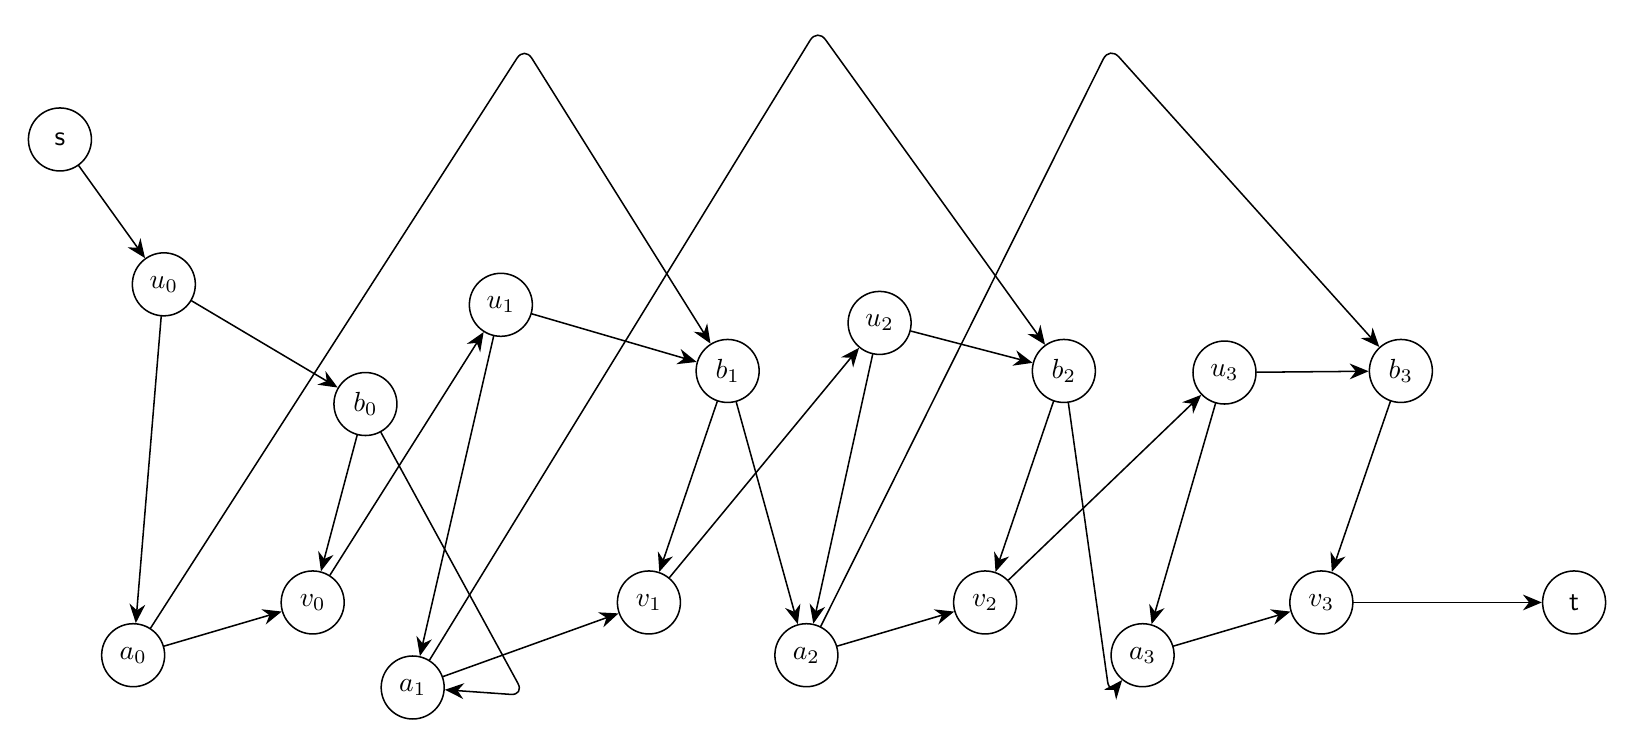
\begin{tikzpicture}[x=1cm,y=1cm]
\tikzset{
  graphnode/.style={circle,draw=black,line width=0.55pt,minimum size=8mm,inner sep=1pt,font=\sffamily},
  graphedge/.style={draw=black,line width=0.55pt,line cap=round,line join=round},
  directed/.style={graphedge,-{Stealth[length=2.4mm,width=2.0mm]}},
  undirected/.style={graphedge}
}
\node[graphnode] (n_s) at (-9.52,3.13) {s};
\node[graphnode] (n_t) at (9.71,-2.75) {t};
\node[graphnode] (n_u_0) at (-8.20,1.29) {$u_{0}$};
\node[graphnode] (n_v_0) at (-6.31,-2.75) {$v_{0}$};
\node[graphnode] (n_a_0) at (-8.59,-3.42) {$a_{0}$};
\node[graphnode] (n_b_0) at (-5.64,-0.23) {$b_{0}$};
\node[graphnode] (n_u_1) at (-3.92,1.03) {$u_{1}$};
\node[graphnode] (n_v_1) at (-2.04,-2.75) {$v_{1}$};
\node[graphnode] (n_a_1) at (-5.04,-3.83) {$a_{1}$};
\node[graphnode] (n_b_1) at (-1.04,0.19) {$b_{1}$};
\node[graphnode] (n_u_2) at (0.89,0.80) {$u_{2}$};
\node[graphnode] (n_v_2) at (2.23,-2.75) {$v_{2}$};
\node[graphnode] (n_a_2) at (-0.04,-3.42) {$a_{2}$};
\node[graphnode] (n_b_2) at (3.23,0.19) {$b_{2}$};
\node[graphnode] (n_u_3) at (5.27,0.17) {$u_{3}$};
\node[graphnode] (n_v_3) at (6.50,-2.75) {$v_{3}$};
\node[graphnode] (n_a_3) at (4.23,-3.42) {$a_{3}$};
\node[graphnode] (n_b_3) at (7.51,0.19) {$b_{3}$};
\draw[directed] (n_u_0) -- (n_a_0);
\draw[directed] (n_u_0) -- (n_b_0);
\draw[directed] (n_a_0) -- (n_v_0);
\draw[directed] (n_b_0) -- (n_v_0);
\draw[directed] (n_u_1) -- (n_a_1);
\draw[directed] (n_u_1) -- (n_b_1);
\draw[directed] (n_a_1) -- (n_v_1);
\draw[directed] (n_b_1) -- (n_v_1);
\draw[directed] (n_u_2) -- (n_a_2);
\draw[directed] (n_u_2) -- (n_b_2);
\draw[directed] (n_a_2) -- (n_v_2);
\draw[directed] (n_b_2) -- (n_v_2);
\draw[directed] (n_u_3) -- (n_a_3);
\draw[directed] (n_u_3) -- (n_b_3);
\draw[directed] (n_a_3) -- (n_v_3);
\draw[directed] (n_b_3) -- (n_v_3);
\draw[directed] (n_s) -- (n_u_0);
\draw[directed] (n_v_0) -- (n_u_1);
\draw[directed] (n_v_1) -- (n_u_2);
\draw[directed] (n_v_2) -- (n_u_3);
\draw[directed] (n_v_3) -- (n_t);
\draw[directed,rounded corners=5pt] (n_a_0) -- (-3.62,4.31) -- (n_b_1);
\draw[directed,rounded corners=5pt] (n_b_0) -- (-3.62,-3.93) -- (n_a_1);
\draw[directed,rounded corners=5pt] (n_a_1) -- (0.10,4.54) -- (n_b_2);
\draw[directed] (n_b_1) -- (n_a_2);
\draw[directed,rounded corners=5pt] (n_a_2) -- (3.81,4.31) -- (n_b_3);
\draw[directed,rounded corners=5pt] (n_b_2) -- (3.81,-3.93) -- (n_a_3);
\end{tikzpicture}
\end{document}
